\documentclass[11pt]{article}
\usepackage[margin=1.5in]{geometry}
\usepackage{graphicx}
\usepackage{float}
\usepackage{parskip}
\usepackage{amsmath}

\usepackage{pgfplots}
\pgfplotsset{width=10cm, compat=1.9}
\usetikzlibrary{angles, quotes}

\begin{document}

\textbf{\Huge Rotational Motion}

Athan Zhang \& Jeffrey Chen

\section{Rotational Kinematics}

We've previously dealt exclusively with translational motion. However, we know that rotational motion is all around us. From molecules to galaxies, many things rotate about some axis. The study of rotation, however, is analogous to the study of linear motion. 

Imagine a disk rotating about a fixed axis perpendicular to the disk and through its exact center. Points near the rim move faster than points near the axis. However, when points near the rim move through a complete circle, so do any other point on the disk. The angle through which disk rotates is a characteristic of the disk as a whole, as is the rate at which the angle changes.

\subsection{Angular Displacement}
Consider a typical particle on the disk. Let $r_i$ be the distance from the disk's center to the $i$th particle, and $\theta_i$ be the angle measured counterclockwise from a fixed reference line in space to a line from the circle's center to the particle. As the disk rotates through an angle $d\theta$, the particle moves through a circular arc of length 
\begin{align*}
    ds_i = r_i|d\theta|
\end{align*}
Where $d\theta$ is measured in radians, the distance $ds_i$ varies from particle to particle, but the angle $d\theta$ is called the \textbf{angular displacement} and is the same for all particles of the disk. For one complete revolution, the arclength is $2\pi r$ and the angular displacement $\Delta\theta$ is 
\begin{align*}
    \Delta\theta = \frac{2\pi r_i}{r_i} = 2\pi \text{rad} = 360^{\circ} = 1 \text{rev}
\end{align*}

\subsection{Angular Velocity}
The time rate of change of the angle, $d\theta/dt$ is the same for all particles of the disk and is called the \textbf{angular velocity} of the disk.
\begin{align*}
    \omega = \frac{d\theta}{dt}
\end{align*}
For counterclockwise rotation, $\theta$ increases, so $\omega$ is positive. For clockwise rotation, it is the opposite. The units of $\omega$ are radians per second. Since radians are dimensionless, the dimensions of angular velocity are those of reciprocal time ($T^{-1}$).

\subsection{Angular Acceleration}

Just like in linear kinematics, we still have acceleration. The time rate of change of angular velocity is called the \textbf{Angular Acceleration}.
\begin{align*}
    \alpha = \frac{d\omega}{dt} = \frac{d^2 \theta}{dt^2}
\end{align*}

\subsection{Conversion to Tangentials}

At any given point on the disk, we can convert from angular kinematics to tangential kinematics simply by multiplying by $r_i$. 
\begin{align*}
    v_{i,\text{tangent}} = \frac{ds_i}{dt} = \frac{r_i d\theta}{dt} = r_i \omega \\
\end{align*}
and similarly,
\begin{align*}
    a_{i,\text{tangent}} = \frac{dv_i}{dt} = r_i\frac{d\omega}{dt} = r_i \alpha
\end{align*}
Each particle on the disk also has a radial acceleration alongside its tangential acceleration. We've learned this previously as the centripetal acceleration.
\begin{align}
    a_{i,\text{centripetal}} = \frac{v_{i,t}^{2}}{r_i} = \frac{(r_i \omega)^2}{r_i} = r_i \omega^2
\end{align}

\subsection{Constant Angular Acceleration Kinematic Equations (CAAKE)}

Just like how we had the Constant Acceleration Kinematic Equations (CAKE) in linear kinematics, we have the CAAKE equations (with two A's because we love cake) in rotational kinematics. All we have to do is substitute the respective linear quantities with angular quantities.

\begin{table}[H]
    \centering
    \begin{tabular}{c|c}
        Kinematic Equation & Missing Variable \\
        \hline
        $\omega = \omega_{0} + \alpha t$ & $\Delta \theta$ \\
        $\Delta \theta = \frac{1}{2}(\omega + \omega_{0})t$ & $\alpha$ \\
        $\Delta \theta = \omega_{0}t + \frac{1}{2}\alpha t^{2}$ & $\omega$ \\
        $\omega^{2} = \omega_{0}^{2} + 2\alpha\Delta \theta$ & $t$ \\
    \end{tabular}
\end{table}

\section{Rotational Dynamics}

We've talked about Rotational Kinematics, but what are the rotational analogs to linear force and mass? Once again, it depends on which particle we act upon in a spinning disk and the direction. 

\subsection{Torque and Moment of Inertia}

The perpendicular distance between the line of action of a force and the axis of rotation is called the \textbf{lever arm} $\ell$ of the force. A force times its lever arm is the magnitude of the \textbf{torque, $\tau$}, which is the rotational analog to force.
\begin{align*}
    \tau_i = F_i \ell
\end{align*}
Torque can be thought of as a twist, just as a force is thought of as a push. It is the torque that affects the angular velocity of the object. 

The lever arm of the force is $\ell = |r_i \sin\phi_i|$, where $\phi_i$ is the angle between $\Vec{F_i}$ and the position vector $\Vec{r_i}$ from the center to the $i$th particle. The torque can then be calculated as
\begin{align*}
    \tau_i &= F_i r_i \sin\phi_i \\
    &= (F_i \sin\phi_i)r_i \\
    &= F_{i,\text{tangent}} r_i \\
    &= (ma_{i,\text{tangent}})r_i \\
    &= (mr_i \alpha)r_i \\
    &= m_i r_i^2 \alpha \\
\end{align*}

If we sum this value across all particles on a rotational disk, we get
\begin{align*}
    \sum_i \tau_i = \sum_i m_i r_i^2 \alpha
\end{align*}

For a rigid body, that is, all points stay the same distance relative to each other during motion, and the angular acceleration is the same for all particles. Thus, it can be taken out of the sum. The following quantity $\Sigma m_i r_i^2$ is called the \textbf{moment of inertia, I} and is the rotational analog to mass. 

For a continuous object, we use an integral. For a system of particles, we use a sum.

Thus, \textbf{Newton's Second Law for Rotation} can be written as
\begin{align*}
    \tau_{\text{net,ext}} = I\alpha
\end{align*}

\section{Calculating the Moment of Inertia}

\subsection{Systems of Particles}

For systems consisting of discrete particles, we can compute the moment of inertia about a given axis. Using the definition of the moment of inertia,

\begin{align*}
    I = \sum_i m_i r_i^2 
\end{align*}

Keep in mind that $r_i$ varies based on what axis of rotation we are using. For example, if we had two circular balls in space, we would have different moments of inertia for an axis through the two balls and the axis between the two balls.

\subsection{Continuous Objects}
To calculate the moment of inertia for continuous objects, we use an integral. This is because we can think of a continuous object as an infinite sum of infinitely tiny particles. The following table gives the moment of inertia for commonly used objects in problems.

\begin{align*}
    I = \int r^2 dm 
\end{align*}

\begin{figure}[H]
    \centering
    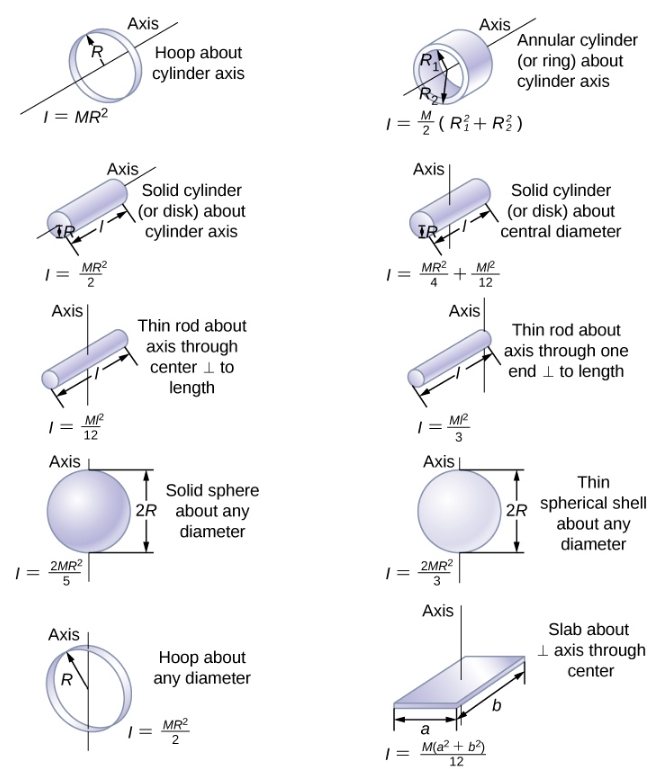
\includegraphics[width=0.7\textwidth]{Physics/images/physics_moments_of_inertia.png}
\end{figure}

\subsection{Parallel-Axis Theorem}

We can often simplify the calculation of moments of inertia for various bodies by using the parallel-axis theorem, which relates the moment of inertia about an axis through the center of mass of an object to the moment of inertia about second, parallel axis. 
\begin{align*}
    I = I_{cm} + MR^2
\end{align*}

\section{Rotational Kinetic Energy}

The kinetic energy of a rotating object is the sum of the kinetic energies of the individual particles in the object. The kinetic energy of a mass element $m_i$ is
\begin{align*}
    K = \frac{1}{2}m_i v_i^2
\end{align*}
When we sum over all elements, we get
\begin{align*}
    K_{\text{rot}} = \frac{1}{2}I\omega^2
\end{align*}

\section{Rolling without Slipping}
Consider a ball of radius $R$ rolling without slipping along a plane surface. As the ball turns through an angle $\phi$, the point of contact between the ball and the plane moves a distance $s$ calculated by
\begin{align*}
    s = R\phi
\end{align*}

Since the ball's center of mass lies directly over the point of contact, it also moves through $s$. The velocity of the center of mass is, therefore
\begin{align*}
    v_{cm} = \frac{ds}{dt} = R\frac{d\phi}{dt}
\end{align*}
or simply,
\begin{align*}
    v_{cm} = R\omega
\end{align*}
and
\begin{align*}
    a_{cm} = R\alpha
\end{align*}
This gives the required nonslip conditions. If these two values are not equal, then we know the object of interest is rolling with slipping.

The Kinetic Energy of a rolling object is
\begin{align*}
    K = \frac{1}{2}Mv_{cm}^2  + \frac{1}{2}I_{cm}\omega^2
\end{align*}

\end{document}